\documentclass{article}
\usepackage{graphicx} % Required for inserting images
\usepackage{amsthm,amsmath,amssymb}
\usepackage{mathrsfs}
\usepackage{float}
\usepackage{blkarray}
\usepackage{authblk}
\usepackage{hyperref}

\title{A Note on the Wigner Semicircle Law}
\author[1]{She Yuting \\
Supervised by: Prof. Yao Jianfeng (CUHKSZ)}
\date{June 2024}

\begin{document}

\maketitle
\section{Introduction}
This note intends to give a proof to Wigner's Semicircle Law on the Wigner matrices. We first explore some important properties of the Wigner matrix, then examine the behaviour of the empirical spectral distribution of a sequence of Hermitian matrix ensembles\\
\\
\textbf{Definition 1.1.1 Wigner Matrix}
 A random matrix ensemble $M_n = (\mathcal{C}_n)_{1 \leq i,j \leq n}$ is called a Hermitian Wigner matrix ensemble, if $M_n$ is Hermitian ($M_n = M_n^{*}$, where * denotes the transpose conjugate of $M_n$), in which the upper triangular coefficients $\mathcal{C}_{ij}$ being jointly independent with
 \begin{itemize}
     \item[(a)] The diagonal entries $\mathcal{C}_{i,i}$ being real i.i.d with mean 0 and
     \item[(b)] The strictly upper triangular entries $\mathcal{C}_{i, j}$, i $<$ j being complex with mean 0 and $\mathbb{E}|\mathcal{C}_{i,j}|^2 = 1$.
 \end{itemize}
 
 One important observation is that all the eigenvalues for a Hermitian matrix are real so it will be sufficient to consider the real eigenvalues of a Wigner matrix $M_n$. Suppose there are n random eigenvalues which we will denote by 
\begin{center}
    $\lambda_1(M_n) \geq \lambda_2(M_n) \geq ... \geq \lambda_n(M_n)$
\end{center}
 In fact (which will be shown later): these are continuous functions of $M_n$ hence they are random variables themselves. In order to observe the bounded property of the eigenvalues of Wigner matrices, we introduce:\\
 \\
\textbf{Definition 1.1.2 The Empirical Spectral Distribution}
 Given any $n\times n$ Hermitian matrix M, we can define the empirical Spectral Distribution (ESD) of M as the normalised counting measure of all the eigenvalues.
 \begin{center}
     $\mu_{M_n} := \frac{1}{n} \sum\limits_{j = 1}^{n} \delta_{\lambda_j(M_n)}$
 \end{center}
where $\lambda_1(M_n) \geq \lambda_2(M_n) \geq ... \geq \lambda_n(M_n)$, with $\delta_{\lambda_j(X_n)}(x)$ being the indicator function $\textbf{1}_{\lambda_j(X_n) \leq x}$.\\
 \\
This $\mu_{M_n}$ is a random discrete probability measure which puts $\frac{1}{n}$ mass to each (random) eigenvalue. Now consider the behaviour of ESD of a sequence of Hermitian matrix ensembles $M_n$ as $n\rightarrow \infty$. \\
By plotting the histogram of the Hermitian matrix with mean 0 and variance 1, we observe that: \\
\begin{figure}[h]
	\begin{minipage}{0.32\linewidth}
		\vspace{3pt}
		\centerline{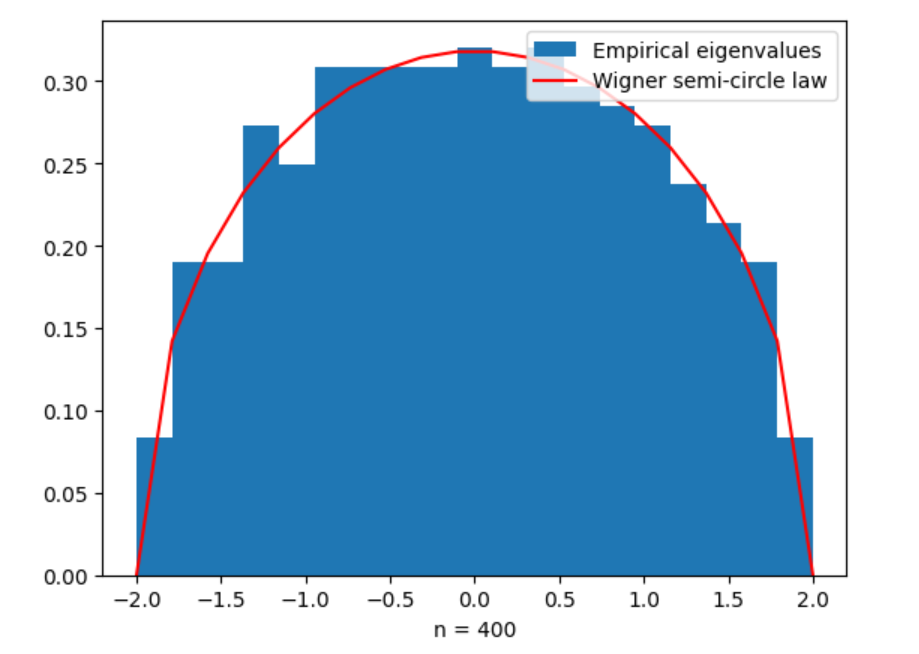
\includegraphics[width=\textwidth]{Screenshot 2024-07-20 223652.png}}
		\centerline{n=400}
	\end{minipage}
	\begin{minipage}{0.32\linewidth}
		\vspace{3pt}
		\centerline{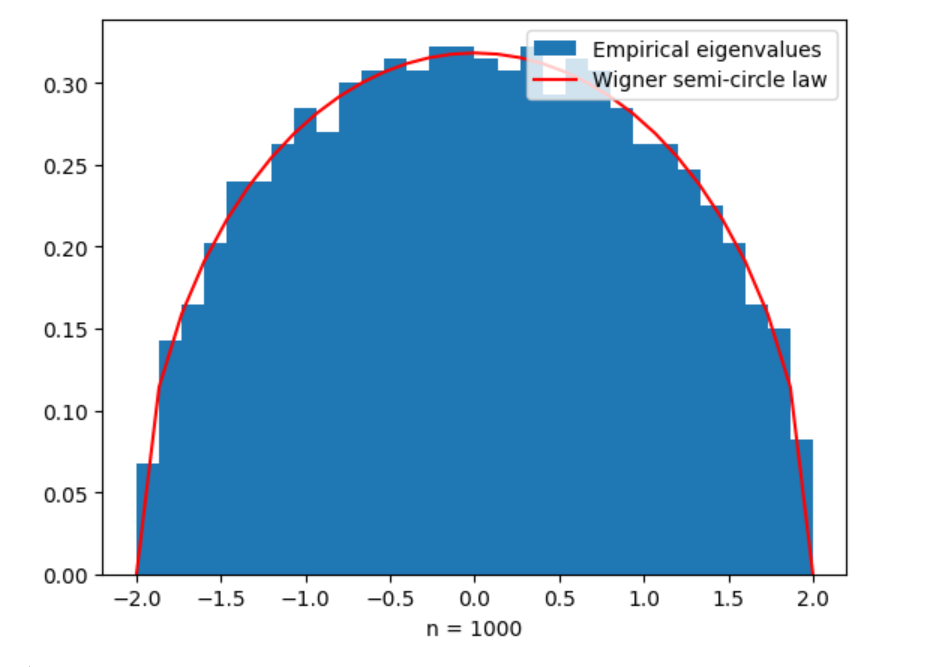
\includegraphics[width=\textwidth]{Screenshot 2024-07-20 223801.png}}
		\centerline{n=1000}
	\end{minipage}
	\begin{minipage}{0.32\linewidth}
		\vspace{3pt}
		\centerline{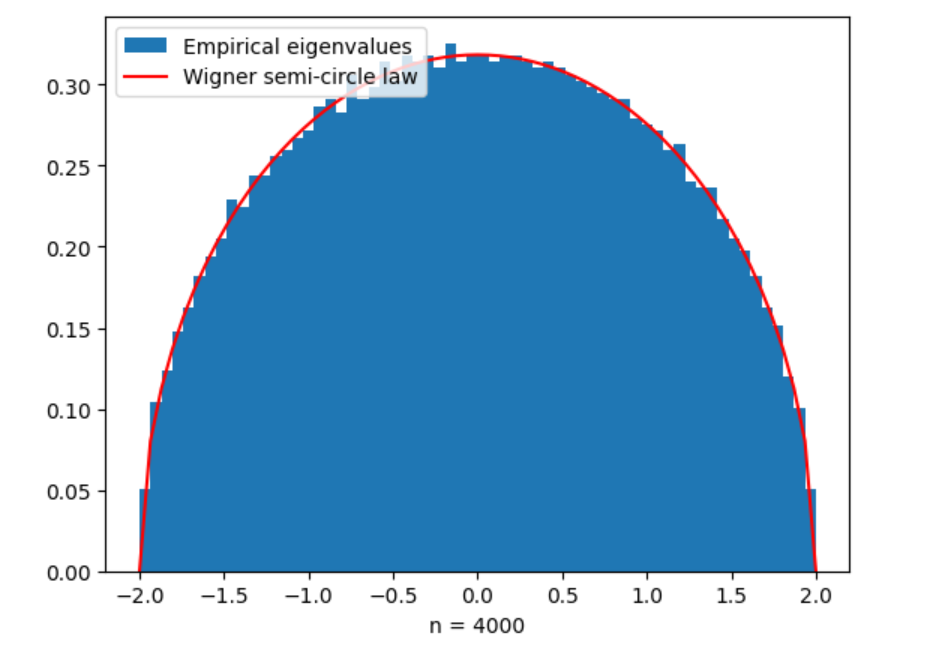
\includegraphics[width=\textwidth]{Screenshot 2024-07-20 224026.png}}
		\centerline{n=4000}
	\end{minipage}
 
	\caption{Histogram of the eigenvalue distribution of Hermitian matrix with mean 0 and unit variance}
\end{figure}
 
 We see that as the size of n increases, a semicircle pattern is observed. The semi-circle law is then, to prove that the distribution of ESD sequence, after proper normalization, indeed converges to a deterministic distribution.

 \section{Convergence of Measures}
 In order to prove that the distribution of ESD converges, we need to firstly define the convergence concept for random measures. \\
 \\
\textbf{Definition 2.3.1} If $\{\mu_n\}_{n \geq 1}$ is a sequence of random measures on $(\mathcal{R}, \mathcal{B}(\mathcal{R}))$, we say $\{\mu_n\}_{n \geq 1}$ converges \textit{weakly} to a deterministic measure $\mu$ if for every compactly supported (bounded) continuous function $f$, \\
\\
\centerline{$\lim\limits_{n \rightarrow \infty} \int_{\mathcal{R}}f d\mu_n = \int_{\mathcal{R}}f d\mu$}
\\
\\
Since the sequence $\{\mu_n\}_{n \geq 1}$ is itself random, if\\
\\
\centerline{$P(\lim\limits_{n \rightarrow \infty} \int_{\mathcal{R}}f d\mu_n = \int_{\mathcal{R}}f d\mu) = 1$}
\\
\\
the sequence is said to converge \textit{\textbf{almost surely}} to a probability measure $\mu$.
\subsection{Normalization of $M_n$}
Intuitively we can understand the scaling factor $\frac{1}{\sqrt{n}}$ by considering convergence of the moments of the Hermitian matrix $M_n$. \\ \\
In general, if the first and the second moment of a random variable converges, then the expectation and the variance of a random variable converges. \\ \\
In particular, we look at the first and second moment of $M_n$. The following are some useful results from linear algebra:\\
\\
\textbf{Theorem 2.3.2} For a Hermitian matrix A, 
\begin{center}
    A = $U^* \Lambda U = \sum\limits_{j = 1}^N \lambda_j u_j u_j^*$
\end{center}
where $\Lambda = $
$\begin{blockarray}{lcccc}
\begin{block}{l(cccc)}
 & \lambda_1 &          &        & \\
 &           &\lambda_2 &        & \\
 &           &          & \ddots &  \\
 &           &          &        &\lambda_n\\
\end{block}
\end{blockarray}$
and U is a unitary vector with $\{ u_i \}$ being the orthonormalised eigenvector for each corresponding engenvalue $\{ \lambda _i\}$.
\\
\\
\noindent\textit{Proof:} This result follows immediately from the Principal Axis Theorem. Note that all Hermitian matrices are normal matrices. \\
\\
\textbf{Proposition 2.3.3} Let $A = (a_{i,j})_{n \times n}$ and $B = (b_{i,j})_{n \times n}$ be real or complex square matrices. Then
\begin{center}
    Tr(AB) = Tr(BA) = $\sum\limits_{i = 1}^n \sum\limits_{j = 1}^n a_{i,j}b_{j,i}$.
\end{center}
This is true because the dimension of A, B are fixed, so the sums are commutative to each other.
\\ \\
It then follows that given matrix $M_n$ = $U^*\Lambda U$, we have
\begin{center}
    Tr($M_n$) = Tr($U^* \Lambda U$) = Tr($\Lambda U^*U$) = Tr($\Lambda$) = $\sum\limits_{i = 1}^n \lambda_i$
\end{center}
\textbf{Corollary 2.3.4} Assume that A is diagonalizable. Then for any integer k$\geq$0,
\begin{center}
    Tr($A^k$) = $\sum\limits_{i = 1}^n \lambda^k$
\end{center}
with a simple induction on Proposition 1.3.5.
\\
\\
The first moment of $M_n$ is thus
\begin{center}
    $\frac{1}{n} \sum\limits_{i = 1}^n \lambda_i = Tr(M_n) = \sum\limits_{i = 1}^n \mathcal{C}_{i,i}$
\end{center}
and the second moment of $M_n$ is
\begin{center}
    $\frac{1}{n} \sum\limits_{i = 1}^n \lambda_i^2$ = $Tr(M_n ^ 2)= \sum\limits_{i = 1}^n \sum\limits_{j = 1}^n \mathcal{C}_{i,j}^2$ = $\frac{1}{n} (\sum\limits_{i = 1}^n \mathcal{C}_{i,i}^2 + 2\sum\limits_{i < j}\mathcal{C}_{i, j}^2)$
\end{center}
And it is easy to see that the first and second moments of $M_n$ converges: \\
It is clear that the first moment converges to 0 by the strong law of large numbers.\\
For the second moment, since $\frac{1}{n} \sum\limits_{i = 1}^n \mathcal{C}_{i,i}^2 \rightarrow 0$ as $n \rightarrow \infty$, by the law of large numbers (as $\mathbb{E} [\mathcal{C}_{i,i} ^ 2] = 1$ by definition), we are then interested in the convergence of the term $\frac{2}{n}\sum\limits_{i < j}\mathcal{C}_{i, j}^2$.\\
\\
Similarly, by the law of large numbers we know that: \\
\\
\centerline{$\lim\limits_{n \rightarrow \infty}\frac{1}{\frac{n(n - 1)}{2}}\sum\limits_{i < j}\mathcal{C}_{i, j}^2 = l$ for some $l \in \mathbb{R}^+, l < \infty$}
\\
\\
therefore as $n \rightarrow \infty$,\\
\begin{align*}
    \lim\limits_{n \rightarrow \infty}\frac{2}{n}\sum\limits_{i < j}\mathcal{C}_{i, j}^2 = \lim\limits_{n \rightarrow \infty}\frac{2}{n} \frac{n (n-1)}{2} \frac{1}{\frac{n (n-1)}{2}}\sum\limits_{i < j}\mathcal{C}_{i, j}^2 = n l
\end{align*}
\\
which is of O(n). This suggests that in order to see a meaningful limit, we need to scale the eigenvalues (or the matrix) by $\frac{1}{\sqrt{n}}$.\\
Although this argument is far from being rigorous, it provides an insight to how we can understand the scaling factor. Since a rigorous proof of this bound involves discussions of the measure concentration, we defer the proof to Annex A after we explore more properties of the measure concentrations (i.e the Talagrand's inequality).

\section{Eigenvalue Distribution of Wigner Matrices}
 \subsection{The Semicircle Law} 
 \textbf{Definition 3.1.1} Let $M_n$ be the top left $n \times n$ minors of an infinite Wigner matrix $(\mathcal{C})_{i,j \geq 1}$. Then the ESDs $\mu_{\frac{1}{\sqrt{n}} M_n}$ converge almost surely (and hence also in probability and expectation) to the Wigner semicircular distribution:
 \begin{center}
     $\mu_{sc} := \frac{1}{2\pi} \sqrt{4 - x^2}$
 \end{center}
 There are several ways to establish the semicircular law, including the moment method, Stieltjes transform method, free probability method as well as the Dyson Brownian motion method. Stieltjes transform is considered one of the most powerful and accurate tools in dealing with the ESD of random Hermitian matrices.\\
 The basic starting point of both moments and the Stieltjes transform method, however, starts from the observation that the moments of the ESD can be written as normalised traces of powers of $M_n$:
 \begin{center}
     $\int_{\mathbb{R}} x^k d\mu_{\frac{1}{\sqrt{n}}M_n}(x) = \frac{1}{n}Tr(\frac{1}{\sqrt{n}}M_n)^k$.
 \end{center}
 In particular, on taking expectations, we have
 \begin{center}
     $\int_{\mathbb{R}} x^k d\mathbf{E}[\mu_{\frac{1}{\sqrt{n}}M_n}(x)] = \mathbf{E}\left[\frac{1}{n}Tr(\frac{1}{\sqrt{n}}M_n)^k\right]$.
 \end{center}
 \subsection{The Stieltjes Transform Method}
 When dealing with random Hermitian matrices, we use Stieltjes transform to characterize the (normalized) ESD proceeding from the identity:
 \begin{center}
     $\int_{\mathcal{R}} \frac{1}{x - z} d\mu_{\frac{1}{\sqrt{n}} M_n}(x)$ = $\frac{1}{n} \sum\limits_{i=1}^n \frac{1}{\lambda_i (\frac{1}{\sqrt{n}} M_n) - z} d\mu_{\frac{1}{\sqrt{n}} M_n}(x)$ =$\frac{1}{n} Tr(\frac{1}{\sqrt{n}} M_n - zI)^{-1}$
 \end{center}
defined for complex number z outside of the support of $\mu_n$, $z \in \mathbb{C}^+$. \\ \\
We refer to the expression on the left hand side as the \textbf{Stieltjes transform} of $\mu_{\frac{1}{\sqrt{n}} M_n}$, and denote it by $s_{\mu_{\frac{1}{\sqrt{n}} M_n}}$ or as $s_n$ for short.\\
\\
The expression ($\frac{1}{\sqrt{n}} M_n - zI)^{-1}$ is the \textbf{normalised resolvent} of $M_n$, and plays an important role in the spectral theory of that matrix. \\
\\
\textbf{Theorem 3.2.1 Stieltjes Transform} For any probability measure $\mu$ defined on ($\mathbb{R}, \mathcal{B}(\mathbb{R})$), the Stieltjes transform of $\mu$ is
\begin{center}
    $s_\mu (z) = \int_{\mathbb{R}} \frac{1}{x - z} d\mu (x)$
\end{center}
for any $z \notin supp(\mu)$. \\
\\
\textbf{Proposition 3.2.2} Let $\mu$ be a probability measure on $\mathbb{R}$ and $S_{\mu}$ be its Stieltjes transform, then we have the following: 
\begin{itemize}
    \item[(i)] $S_\mu (z) \in \mathbb{C}^+$, i.e. the Stieltjes transform is well-defined on $\mathbb{C}^+$ and 
    \item[(ii)] $S_\mu$ is analytic on $\mathbb{C}^{+} $.
\end{itemize}
where $\mathbb{C}^+ = \{ z \in \mathbb{C} :$ Im(z) $ > 0\}$.
\begin{proof}
    (i) We observe that by writing z $:=$ a + $i$b, Im$\frac{1}{x - z} = \frac{b}{(x - a)^2 + b^2} > 0$ as the reciprocal of a complex number z is given by $\frac{\Bar{z}}{\mid z \mid ^2}$. Therefore we have $S_\mu(z) \in \mathbb{C}^+$.\\
    (ii) A function f(z) is analytic if it has a complex derivative $f'(z)$. Since $\frac{1}{x - z}$ is analytic on $\mathbb{C}^+$, its integral over the real line is also analytic on $\mathbb{C}^+$. \\
\end{proof}
\noindent The imaginary part of Stieltjes transform is of typical interest. It provides a meaning bound for $s_\mu (z)$. By applying conjugations on the Stieltjes transform $s_{\mu}(z)$ we obtain the symmetry: \\
\\
\centerline{$\overline{s_{\mu}(z)}:= s_{\mu}(\Bar{z})$,}
\\
From the trivial bound \\
\\
\centerline{$\mid \frac{1}{x - z} \mid \leq \frac{1}{\mid Im(z) \mid}$}
\\
\\
One has the pointwise bound\\
\\
\centerline{$\mid s_{\mu}(z) \mid \leq \frac{1}{\mid Im(z) \mid}.$}
\\
\\
Actually, we can recover $\mu$ from $S_{\mu}$ using the Stieltjes inversion formula:
\\ \\
\textbf{Theorem 3.2.3 Stieltjes Inversion Formula} For any continuous points $a < b$ of probability measure $\mu$, we have \\
\centerline{$\mu ([a,b])$ = $\lim\limits_{\epsilon \rightarrow 0^+} \frac{1}{\pi} \int_{a}^b Im(s_\mu (x + i \epsilon)) dx.$}
\\
\textit{Proof:} We have
\begin{align*}
    \frac{1}{\pi} \int_a^b Im(s_{\mu} (x + i \epsilon)) dx 
    &= \frac{1}{\pi} \int_a^b \int_{\mathbb{R}} \frac{\epsilon d_{\mu}(y)}{(x - y)^2 + \epsilon^2}dx \\
    &= \frac{1}{\pi} \int_{\mathbb{R}} \int_a^b \frac{\epsilon d_{\mu}(y)}{(x - y)^2 + \epsilon^2}d\mu (y) \text{    (Fubini-Tonelli)}\\
    &= \int_{\mathbb{R}} \frac{1}{\pi} \left[\arctan \left (\frac{b - y}{\epsilon}\right) - \arctan \left (\frac{a - y}{\epsilon} \right)\right]d\mu(y).\\
\end{align*}
Let $\epsilon \rightarrow 0^+$, from the dominating convergence theorem, the right-hand side tends to $\mu([a, b])$.
\\
\\
One can also express the imaginary part of the Stieltjes transform as a convolution:\\
\centerline{Im($s_\mu (a + ib)$) = $\pi \mu$ * $P_b(a)$}
\\
\\
where $P_b(a)$ is the Poisson kernel \\
\\
\centerline{$P_b(a) := \frac{1}{\pi} \frac{b}{x^2 + b^2}$}
\\
\\
The kernels form a family of approximations to the identity, and thus $\mu * P_b$ converges in the vague topology to $\mu$. (i.e $\lim\limits_{b \rightarrow 0^+} (\mu * P_b) = \mu * \delta_0 = \mu$.)\\
Thus we see that \\
\\
\centerline{$Im(s_\mu (a + i\epsilon)) \rightharpoonup \pi \mu$}
\\
\\
as $\epsilon \rightarrow 0^+$, or equivalently suppose that $\mu$ has density $\rho$ at $x \in \mathbb{R}$, we have \\
\\
\centerline{$\rho (x) = \lim\limits_{\epsilon \rightarrow 0^+} Im(s_\mu (x + i \epsilon)) = \lim\limits_{\epsilon \rightarrow 0^+} \frac{s_\mu (x + i\epsilon) - s_\mu (x - i\epsilon)}{2\pi i} = d\mu(x)$}
\\
\\
Thus we see that a probability measure $\mu$ can be recovered in terms of limiting behaviour of Stieltjes transform on the real axis. \\
\\
\textbf{Theorem 3.2.4 Stieltjes Continuity Theorem, deterministic} Let $\{\mu_n\}_{n \geq 1}$ be a sequence of \textit{deterministic} probability measures on the real line, and let $\mu$ be a deterministic probability measure. Then $\mu_n$ converges in the vague topology to a probability measure $\mu$ if and only if \\
\\
\centerline{$\lim\limits_{n \rightarrow \infty} s_{\mu_n}(z) = s_{\mu}(z), \forall z \in \mathbb{C}^+$.}
\\
\\
\textbf{Theorem 3.2.5 Stieltjes Continuity Theorem, random} Let $\{\mu_n\}_{n \geq 1}$ be a sequence of \textit{random} probability measures on the real line, and let $\mu$ be a deterministic probability measure. Then $\mu_n$ converges in the vague topology to a probability measure if and only if \\
\\
\centerline{$ s_{\mu_n}(z) \stackrel{a.s.}{\longrightarrow} s_{\mu}(z), \forall z \in \mathbb{C}^+$.}
\\
\\
We will proceed the Stieltjes transform method in the following 2 steps:
\begin{itemize}
    \item[1.] For any fixed $z \in \mathbb{C}^+$, $s_n(z) - \mathbb{E}[s_n(z)] \stackrel{a.s.}{\longrightarrow} 0$
    \item[2.] For any fixed z$\in \mathbb{C}^+, \mathbb{E}[s_n(z)] \rightarrow s_{sc}(z)$, the Stieltjes transform of the semicircle distribution.
\end{itemize}

\section{Measure Concentration of $s_n(z)$}
In this section, we show that for any fixed $z \in \mathbb{C}^+$, $s_n(z) - \mathbb{E}[s_n(z)] \stackrel{a.s.}{\longrightarrow} 0$.\\
The main idea is to compare the transform $s_n(z)$ of the $n \times n$ matrix $M_n$ with the transform $s_{n - 1}(z)$ of the top left $ n-1 \times n-1$ minor $M_{n-1}$. It is ideal to have (and will be proven later) that an extra row or column has only a limited amount of influence on the Stieltjes transform $s_n(z)$, then a standard measure concentration result can be applied to control the deviation of $s_n(z)$ from $\mathbb{E}[s_n(z)]$.\\
\\
We start with an important relationship between the eigenvalues of the two matrices.
\subsection{Bounded Total Variation of $s_n(z)$}


\textbf{4.1.1 Cauchy Interlacing Law} For any $n\times n$ Hermitian matrix $A_n$ with top left $n-1 \times n-1$ minor $A_{n-1}$, we have:\\
$\lambda_1(A_n) \geq \lambda_1 (A_{n-1}) \geq \lambda_2(A_n) \geq \lambda_2 (A_{n-1})$...$\lambda_{n-1}(A_n) \geq \lambda_{n-1}(A_{n-1}) \geq \lambda_n (A_n)$.
\begin{proof}
WLOG, we can reorder the columns of $A_n$ so that we always have $\lambda_n \leq \lambda_{n-1} \leq ... \leq \lambda_1$.
Note that matrix $A_n$ is of the form \\
\begin{center}
    $A_n$ = $
\left(
\begin{array}{ccc}
A_{n-1} &y^* \\
y &a_{nn}
\end{array}
\right) $.
\end{center}
where * signifies the conjugate transpose of a matrix. Let D = $diag(\mu_1, \mu_2,..., \mu_{n-1})$, where $\mu_i := \lambda_{i}(A_{n-1})$. Then since $A_{n-1}$ is also Hermitian, there exists a unitary matrix U of order $n - 1$ such that $U^* A_{n-1}U = D$. Let $U^*y = z = (z_1, z_2, ..., z_{n-1})^T$.\\
Let
\begin{center}
    V = $
\left(
\begin{array}{ccc}
U &0^* \\
0 &1
\end{array}
\right) $,
\end{center}
in which 0 denotes the zero vector. Then V is a unitary matrix and
\begin{center}
    $V^*AV$ = $
\left(
\begin{array}{ccc}
D &z^* \\
z &a_{nn}
\end{array}
\right) $.
\end{center}
Let $f(x) = det(xI-A)= det(xI- V^*AV)$, where \textit{I} denotes the identity matrix, expanding $det(xI - V^*AV)$ along the last row, we get:\\
\\
\centerline{$f(x) = (x-a)(x-\mu_1)...(x - \mu_{n-1})-\sum\limits_{i = 1}^{n-1} f_i(x)$.}
\\
\\
where $f_i(x) = \left| z_i^2 \right| (x - \mu_1)...(x - \mu_{i-1})(x - \mu_{i+1})...(x - \mu_{n-1})$ for $i = 1, 2, ..., n-1$.\\
Note that $f_i(\mu_j) = 0$ if $j \neq i$ and that \\
\[ f_i(\mu_i) = \begin{cases} 
      >0 & \text{if i is even} \\
      <0 & \text{if i is odd}
   \end{cases}
\]
\\
Hence that \\
\[ f(\mu_i) = \begin{cases} 
      <0 & \text{if i is even} \\
      >0 & \text{if i is odd}
   \end{cases}
\]
\\
for $i = 1, 2, ..., n-1$. Since $f(x)$ is a polynomial of degree n with positive leading coefficient, the intermediate value theorem ensures the existence of n roots $\lambda_1, \lambda_2,..., \lambda_n$ of the equation $f(x) = 0$ such that $\lambda_n \leq \mu_{n-1} \leq \lambda_{n-1} \leq ... \leq \lambda_2 \leq \mu_1 \leq \lambda_1$.\\
\end{proof}
\noindent Now for $z = a + ib$, $b > 0$, let $f(x) = Im\left(\frac{1}{x - z}\right) = \frac{b}{(x-a)^2 + b^2}$, then $0 < f(x) \leq \frac{1}{b}$. The main idea here is to compare the transform $s_n(z)$ of the $n \times n$ matrix $M_n$ and $s_{n-1}(z)$ of the $n-1 \times n-1$ minor $M_{n-1}$. Together with the fact that $f$ is decreasing, the function has bounded total variation:\\
for any $a_0 < ... < a_m$, 
\begin{center}
    $\sum\limits_{k=1}^m \left| f(a_k) - f(a_{k-1})\right| = \left| f(a_0) - f(a_{n})\right| \leq \frac{2}{b}$
\end{center}
Then
    \begin{align*}
         & \left| \sum\limits_{j = 1}^n \frac{b}{\left(\frac{\lambda_j (M_n)}{\sqrt{n}} - a \right)^2 + b^2} - \sum\limits_{j = 1}^{n-1} \frac{b}{ \left(\frac{\lambda_j( M_{n-1})}{\sqrt{n}} - a\right)^2 + b^2}
        \right|\\
        =&\left| \sum\limits_{j = 1}^n f \left(\frac{\lambda_j(M_n)}{\sqrt{n}} \right) - \sum\limits_{j = 1}^{n-1} f \left(\frac{\lambda_j(M_{n-1})}{\sqrt{n}} \right)
        \right| \\
        \leq &\sum\limits_{j = 1}^{n-1} \left|f \left(\frac{\lambda_j(M_n)}{\sqrt{n}} \right) - f \left(\frac{\lambda_j(M_{n-1})}{\sqrt{n}} \right)
        \right| + \left| f \left(\frac{\lambda_n(M_n)}{\sqrt{n}} \right) \right| \\
        \leq &\frac{3}{b}
    \end{align*}
Hence
\begin{center}
    $\left|nIm(s_n(a + ib)) - \sqrt{n(n-1)}Im(s_{n-1} \left(\frac{\sqrt{n}}{\sqrt{n - 1}}(a+ib)\right)\right| \leq \frac{3}{b}$
\end{center}
Then
\begin{center}
    $\left|Im(s_n(a + ib)) - Im(s_{n-1}(a+ib))\right| = O\left(\frac{1}{n}\right)$
\end{center}
Similarly, by writing $g(x) = Re\left(\frac{1}{x - z}\right) = \frac{x-a}{(x-a)^2 + b^2}$, we have:
\begin{center}
    $\left|Re(s_n(a + ib)) - Re(s_{n-1}(a+ib))\right| = O\left(\frac{1}{n}\right)$
\end{center}
Hence
\begin{center}
    $\left|s_n(a + ib) - s_{n-1}(a+ib)\right| = O\left(\frac{1}{n}\right)$
\end{center}
Observe that while $s_n(z)$ is dependent on the $n\times n$ matrix $M_n$, $s_{n-1}(z)$ is only dependent on $n-1 \times n-1$ minor of that matrix. In particular this suggests independence of the n-th row and column of $M_n$. That suggests the entire row and column have limited influence on the Stielejes transform $s_n(z)$. And by permuting the rows and columns, we know that any row or column of $M_n$ influence $s_n(z)$ at most $O\left(\frac{1}{n}\right)$.\\
\\
By treating $s_n(z)$ as a n-variate function of the rows of $M_n$, since all the rows are independent, the following result on measure concentration is applicable.

\subsection{Convergence of $s_n(z)$}
Before proving the convergence of $s_n(z)$, we prove some useful theorems that are useful in the proof later.\\
\\
\textbf{Theorem 4.2.1 Chernoff Bounds} If X is a random variable, then for any $a \in \mathbb{R}$, we can write
\begin{align*}
    &P(X \geq a) = P(e^{sX} \geq e^{sa}), \text{ for } s > 0, \\
    &P(X \leq a) = P(e^{sX} \geq e^{sa}), \text{ for } s < 0.
\end{align*}
\begin{proof}
    As $e^{sX} > 0$ for all $s\in \mathbb{R}$, for some $s > 0$,
    \begin{align*}
        P(X \geq a) &= P(e^{sX} \geq e^{sa}) \\
                    &\leq \frac{E[e^{sX}]}{e^{sa}} \text{ (by Markov's inequality).}\\
                    &= e^{-sa} M_X(s)
    \end{align*}
    Similarly, for some $s < 0$, 
    \begin{align*}
        P(X \leq a) &= P(sX \geq sa)\\
                    &= P(e^{sX} \geq e^{sa}) \\
                    &\leq \frac{E[e^{sX}]}{e^{sa}}\\
                    &= e^{-sa}M_X({s})
    \end{align*}
\end{proof}
The Chernoff bound is considered a stronger condition compared to the Markov inequality and/or the Chebyshev inequality.\\
\\
\noindent\textbf{Theorem 4.2.2 Hoeffding's Inequality} Consider the sum $S_n = \sum\limits_{i=1}^n X_i$ for independent random variables $X_i$, then we have for all $s > 0$,
\begin{align*}
    P(S_n - \mathbb{E}[S_n] \geq t) &= P(exp(s(S_n - \mathbb{E} [S_n])) \geq e^{st})\\
    &\leq e^{-st} \mathbb{E}\left[ e^{s(S_n - \mathbb{E}[S_n])}\right]\\
    &= e^{-st} \prod\limits_{i=1}^n \mathbb{E}[e^{s(X_i - \mathbb{E}[X_i])}]
\end{align*}
Which is true by direct application of the Markov's inequality and Chernoff bounds.\\
\\
\textbf{Lemma 4.2.3 Hoeffding's Lemma} Let X be any real-valued random variable with expected value $\mathbb{E}[X] = 0$ and such that $a \leq X \leq b$ almost surely, for some $a, b \in \mathbb{R}$, $0 \in [a, b]$. Then for all $s \in \mathbb{R}$,\\
\\
\centerline{$\mathbb{E}[e^{sx}] \leq exp\left( \frac{s^2(b-a)^2}{8}\right)$}
\\
\begin{proof}
    As $e^{sx}$ is convex in x and is this uniformly bounded, i.e.
    \begin{align*}
        e^{sx} &\leq \lambda e^{sb} + (1-\lambda) e^{sa}, \text{ where } \lambda := \frac{x-a}{b-a}\\
        &= \frac{x-a}{b-a}e^{sb} + \frac{b-x}{b-a}e^{sa}
    \end{align*}
    Taking expectation on both sides yields
    \begin{align*}
        \mathbb{E}[e^{sX}] \leq \frac{b}{b-a}e^{sa} - \frac{a}{b-a}e^{sb}
    \end{align*}
    Let $\theta := \frac{b}{b-a}$, $u := s(b-a)$, by taking ln on both sides, on the right hand side we have
    \begin{align*}
        \Phi(u) &= ln(\theta e^{sa} + (1-\theta)e^{sb}) \\
        &= sa + ln(\theta + (1-\theta)e^u) \\
        &= (\theta-1)u + ln(\theta +(1 - \theta)e^u) 
    \end{align*}
    By taking the Taylor's expansion at s = 0, $\exists \xi = \xi(u) \in \mathbb{R}$ s.t. \\
    \\
    \centerline{$\Phi(u) = \Phi(0) + \Phi'(0) + \frac{1}{2} \Phi''(\xi)u^2$}
    \\
    \\
    as $\Phi(0) = 0$ and\\
    \\
    \centerline{$\Phi'(u) = (\theta - 1) + \frac{(1-\theta)e^u}{\theta + (1-\theta)e^u}$}
    \\
    \\
    we have $\Phi'(0) = 0$.
    Hence $\Phi(u) = \frac{1}{2} \Phi''(\xi) u^2$.
    Note that $\Phi''(u)$ is bounded above by a constant number:
    \begin{align*}
        \Phi''(u) &= \frac{\theta (1-\theta)e^u}{(\theta + (1-\theta)e^u)^2}\\
        &= \left(\frac{\theta}{\theta + (1-\theta)e^u}\right) \left(\frac{(1-\theta)e^u}{\theta + (1-\theta)e^u}\right) \\
        &= t(1-t), \text{ where }t :=  \frac{\theta}{\theta + (1 - \theta)e^u}, t \in (0, 1] \\
        &\leq \frac{1}{4}
    \end{align*}
    Thus we have $\Phi(u) \leq \frac{u^2}{8}$, which implies $ln \mathbb{E}[e^{sX}] \leq \frac{s^2(b-a)^2}{8}$ and by taking exponential on both sides, we prove the lemma.\\
\end{proof}
As $M_n$ is a random matrix with entries of known expectations and variances, we expect the variations between iid copies of $M_n$ to be also small and bounded. It turns out that a particularly useful class of a regularity hypothesis here is a Lipschitz hypothesis -- that small variations in $X := (X_1, ..., X_n)$, where $X_i$ are iid distributed random variables, lead to small variations in $F(X)$, which is some combinations of X. This is described by McDiarmid's inequality.\\
\\
\textbf{Theorem 4.2.4 McDiarmid's Inequality} Let $X_1, X_2, ..., X_n$ be independent random elements taking values in range $R_1, R_2, ..., R_n$, and let $F: R_1 \times R_2 \times ... \times R_n \rightarrow \mathbb{C}$ be a function with the property that if one freezes all but the $i^{th}$ coordinate of $F(x_, ..., x_n)$ for some $\leq i \leq n$, the F only fluctuates by at most $c_i > 0$, thus\\
\\
\centerline{$\left| F(x_1, ..., x_{i-1}, x_i, x_{i+1}, ..., x_n) - F(x_1, ..., x_{i-1}, x_i ', x_{i+1}, ... , x_n)\right| \leq c_i$}
\\
\\
for all $x_i \in X_j, x_j ' \in X_i$ for $1 \leq j \leq n$. Then for any $\lambda > 0$, one has \\
\\
\centerline{\textbf{P}$(\left| F(X) - \mathbb{E}F(X)\right| \geq \lambda\sigma) \leq C e^{-c\lambda^2}$}
\\
\\
for some constants $C, c > 0$, where $\sigma^2 := \sum\limits_{i=1}^n c_i^2$.\\
\begin{proof}
    Write $\mathbb{E}_i [.]$ to denote expectation conditioned on $X_{1:i} := (X_1, ..., X_i)$. Therefore, $g_i (X_{1:i}) := \mathbb{E}_i[f(X_{1:n})]$ is a function of $X_{1:i}$. Define the random variables:
    \begin{align*}
        Y_i &:= g_i(X_{1:i}) - g_{i-1}(X_{1:i-1})\\
        A_i &:= \inf\limits_{x_i \in R_i} g_i(X_{1:i-1}, x_i) - g_{i-1}(X_{1:i-1}), \\
        B_i &:= \sup\limits_{x_i \in R_i} g_i (X_{1:i-1}, x_i) - g_{i-1}(X_{1:i-1}).
    \end{align*}
    such that
    \begin{align*}
        &Y_i \in [A_i, B_i],\\
        &\mathbb{E}_{i-1} [Y_i] = 0,\\
        &\sum\limits_{i=1}^{n} Y_i = f(X_{1:n}) - \mathbb{E}[f(X_{1:n})].
    \end{align*}
    Assume that $[A_i, B_i]$ is always an interval of length at most $c_i$. Let $S_i := \sum\limits_{j=1}^i Y_j$, then
    \begin{align*}
        \mathbb{E}[e^{\lambda S_n}] &= \mathbb{E}[e^{\lambda(Y_n + S_{n-1})}] \\
                                    &= \mathbb{E}\left[\mathbb{E}_{n-1}\left[e^{\lambda Y_n}\right]e^{\lambda S_{n-1}}\right] \\
                                    &\leq exp(\lambda^2 c_n^2/8) \mathbb{E}[exp(\lambda S_{n-1})] \\
                                    &= exp(\lambda^2 c_n^2/8)\mathbb{E}[exp(\lambda(Y_{n-1} + S_{n-2}))]\\
                                    &= exp(\lambda^2 c_n^2/8)\mathbb{E}[\mathbb{E}_{n-2}[exp(\lambda Y_{n-1})]exp(\lambda S_{n-2})]\\
                                    &\leq exp(\lambda^2 c_n^2/8)exp(\lambda^2 c_{n-1}^2/8)\mathbb{E}[exp(\lambda S_{n-2})]\\
                                    &\vdots \\
                                    &\leq exp(\lambda^2 c_n^2/8)...exp(\lambda^2 c_1^2/8) \\
                                    &= exp\left(\frac{\sum_{i=1}^n c_i^2}{4} .\frac{\lambda^2}{2}\right)\\
                                    &= Ce^{c\lambda^2}.
    \end{align*}
    By applying the Hoeffding's lemma inductively, where $C = exp(\frac{\sum_{i=1}^n c_i^2}{4})$, $c = \frac{1}{2}$. Observe that $S_n$ is $\frac{\sum_{i=1}^n c_i^2}{4}$-subgaussian.\\
    Now it remains to prove the assumption that $[A_i, B_i]$ is an interval of length at most $c_i$. We show that $B_i - A_i \leq c_i$. By independence of $X_1, ..., X_n$, we have
    \begin{align*}
        g_i(X_{1:i-1}, x_i) &= \mathbb{E}[f(X_{1:i-1},x_i,X_{i+1:n}) | X_{1:i-1};X_i = x_i] \\
        &= \mathbb{E}[f(X_{1:i-1}, x_i, X_{i+1:n}')|X_{1:i-1}]
    \end{align*}
    Where $ X_{i+1:n}'$ is an independence copy of $X_{i+1:n}$. Then
    \begin{align*}
        B_i - A_i &= \sup\limits_{b \in R_i} g_i(X_{1:i-1}, b) - \inf\limits_{a \in R_i} g_i(X_{1:i-1}, a) \\
        &= \sup\limits_{a,b \in R_i} (g_i(X_{1:i-1}, b) - g_i(X_{1:i-1}, a))\\
        &= \sup\limits_{a,b \in R_i} \mathbb{E}[f(X_{1:i-1}, b, X_{i+1:n}') - f(X_{1:i-1}, a, X_{i+1:n}') | X_{1:i-1}]\\
        &\leq \mathbb{E} \left[ \sup\limits_{a,b \in R_i} |f(X_{1:i-1}, b, X_{i+1:n}') - f(X_{1:i-1}, a, X_{i+1:n}')|| X_{1:i-1}\right]\\
        &\leq c_i \text{ (by the bounded difference property of f). }
    \end{align*}
\end{proof}

By theorem 4.2.4, we conclude that
\begin{center}
    $P(|s_n(a+ib) - \mathbb{E}[s_n(a+ib)]| \geq \lambda) \leq Ce^{-cn\lambda^2}$.
\end{center}
for some constants $C, c > 0$ and $\sigma^2 := \sum_{i=1}^n c_i^2$.
Then from the Borel-Cantelli lemma, for any fixed $z \in \mathbb{C}^+$ we have
\begin{center}
    $s_n(z) - \mathbb{E}[s_n(z)] \stackrel{a.s.}{\longrightarrow} 0.$
\end{center}
\section{Recursive Equation of $\mathbb{E}[s_n(z)]$}
In this section, we show that for any fixed $z \in \mathbb{C}^+$, $\mathbb{E}[s_n(z)] \rightarrow s_{sc}(z)$, the Stielejes transform of the semicircular distribution.
\subsection{Properties of $\mathbb{E}[s_n(z)]$}
\textbf{Proposition 5.1.1 Determinant of Block Matrices (Schur Complement)} Let M be a square matrix of finite order $(a+d) \times (a + d)$ that takes the form
\begin{center}
    $M = \left( 
    \begin{array}{cc}
        A &B  \\
        C &D 
    \end{array}
    \right)$
\end{center}
where A $\in \mathbb{C}^{a\times a}$, B $\in \mathbb{C}^{a\times d}$, C $\in \mathbb{C}^{d\times a}$, D$\in \mathbb{C}^{d \times d}$ such that the Schur complement of block A exists in M. Then we have 
\begin{center}
    $det(M) = det(D -CA^{-1}B)det(A)$.
\end{center}
\begin{proof}
    Assume that block A is invertible, consider the Schur complement of A:
    \begin{center}
        $D -CA^{-1}B$.
    \end{center}
    Consider the tranformation \\
    \begin{center}
        $\left( \
        \begin{array}{cc}
        I_a &0\\
        -CA^{-1} &I_d
        \end{array}
        \right)$$\left( 
    \begin{array}{cc}
        A &B  \\
        C &D 
    \end{array}
    \right)$$\left( \
        \begin{array}{cc}
        I_a &-A^{-1}B\\
            0 &I_d
        \end{array}
        \right)$ = $\left( 
    \begin{array}{cc}
        A &0  \\
        0 &D - CA^{-1}B 
    \end{array}
    \right)$
    \end{center}
    
    Note that det$\left( \
        \begin{array}{cc}
        I_a &0\\
        -CA^{-1} &I_d
        \end{array}
        \right)$ and det$\left( \
        \begin{array}{cc}
        I_a &-A^{-1}B\\
        0 &I_d
        \end{array}
        \right)$ both equal to 1, thus
        \\
        \centerline{$det(M) = det(A(D-CA^{-1}B)) = det(A)det(D - CA^{-1}B)$}
\end{proof}
\noindent\textbf{Lemma 5.1.2} Let $A_n \in \mathbb{C}^{n\times n}$, and let $A_{n-1}$ be the top left $n-1 \times n-1$ minor. Suppose that
\begin{center}
$A_n = \left(
\begin{array}{cc}
    A_{n-1} &X  \\
    Y^* &a_{nn} 
\end{array}
\right) $    
\end{center}
and both $A_n, A_{n-1}$ are invertible. Then
\begin{center}
    $[A_n^{-1}]_{nn} = \frac{1}{a_{nn} - Y^* A_{n-1}^{-1}X}$
\end{center}
Where $[A_n^{-1}]_{nn}$ denotes the $(n,n)$ entry of the matrix $A_n^{-1}$. 
\begin{proof}
    By the property of the inverse of an invertible matrix
    \begin{center}
        $A_n^{-1} = \frac{1}{det(A_n)} adj(A_n)$.
    \end{center}
    by using proposition 5.1.1, we have
    \begin{center}
        $[A_n^{-1}]_{nn} = \frac{det(A_{n-1})}{det(A_n)} = \frac{det(A_{n-1})}{det(a_{nn} - Y^* A_{n-1}^{-1}X)det(A_{n-1})} = \frac{1}{a_{nn} - Y^* A_{n-1}^{-1}X}.$
    \end{center}  
\end{proof}
\noindent Applying Lemma 5.1.2 by letting $A_n = \frac{1}{\sqrt{n}}M_n-zI_n$, we obtain the identity
\begin{center}
    $\left(\frac{1}{\sqrt{n}} M_n - zI_n\right)_{nn}^{-1} = \frac{1}{\frac{1}{\sqrt{n}} \mathcal{C}_{nn} -z - \frac{1}{n}X^*(\frac{1}{\sqrt{n}}M_{n-1} -zI_{n-1})^{-1}X}.$
\end{center}
Since the diagonal entries of $\frac{1}{\sqrt{n}}M_n-zI_n$ have identical distribution, it implies
    \begin{align*}
        \mathbb{E}[s_n(z)] &= \mathbb{E}\left[\frac{1}{n}Tr\left(\frac{1}{\sqrt{n}}M_n -zI_n\right)^{-1}\right] \\
        &= \frac{1}{n} \mathbb{E}\left[ \sum\limits_{i=1}^n \left(\frac{1}{\sqrt{n}}M_n - zI_n \right)^{-1}_{ii} \right]\\
        &= n\cdot \frac{1}{n}  \mathbb{E}\left[\left(\frac{1}{\sqrt{n}}M_n - zI_n \right)^{-1}_{nn} \right] \text{ as the diagonal entries of }M_n \text{ are i.i.d distributed}\\
        &= \mathbb{E}\left[\frac{1}{\frac{1}{\sqrt{n}} \mathcal{C}_{nn} -z - \frac{1}{n}X^*(\frac{1}{\sqrt{n}}M_{n-1} -zI_{n-1})^{-1}X}\right].
    \end{align*}
Denote $R := \left(\frac{1}{\sqrt{n}}M_{n-1} -zI_{n-1}\right)^{-1}$. Consider the stochastic quadratic form $\frac{1}{n}X^*RX$. Here we take vector X that only involves entries that are in $M_n$ but not $M_{n-1}$ and so the random matrix R and the vector X are independent. Recall that z has imaginary part b if $z = a+ib$. \\
Furthermore, observe that $|| X^*R X|| = ||R|| \leq |b|^{-1}$ as the magnitude of the denominator here is bounded below by $|b|$. Then the function $F(X) = X^*RX$ is Lipschitz when X is c-Lipschitz (Here we use the reduction that entries of $M_n$ are bounded):
\begin{center}
    $|F(X)-F(Y)| \leq ||F'(u)||\cdot ||X-Y||$
\end{center}
where $X,Y \in \Omega^n$ and $||F'(u)|| = ||F'(X)|| = ||2X^*R||$. To show F is Lipschitz, we only need to have $F'(u)$ to be bounded:
\begin{center}
    $||F'(u)|| = ||2X^*R|| \leq \sup 2||X||\cdot ||R|| \leq \Tilde{c}\sqrt{n}$
\end{center}
We see that the upper bound of $X^*RX$ is $O(\sqrt{n})$ or loosely $o(n)$.\\
Next we wish to show that the expression concentrates around its expectation. We prove this using the Talagrand's inequality.

\subsection{The Talagrand's Concentration Inequality}
\textbf{Definition 5.2.1 Hamming Distance} Let $\Omega$ be a set equipped with the $\sigma-$field $\mathcal{A}$, for each vector w = $(w_1, w_2,..., w_n) \in \mathbb{R}^n_+$, the weighted Hamming distance between two vectors $x = (x_1, ..., x_n)$, $y = (y_1,...,y_n)$, $x,y \in \Omega^n$ is defined as\\
\centerline{$d_w(x, y) := \sum\limits_{i \leq n} w_i h_i(x,y)$      where $h_i(x,y) = \begin{cases} 
      1 & \text{ if }x_i \neq y_i \\
      0 & \text{ otherwise}
   \end{cases}$}
\\
For a subset A of $\chi^n$, the distances $d_w(x, A)$ and D(x, A) are defined by
\begin{align*}
    &d_w(x, A) := \inf\{y \in A: d_w(x,y)\}\\
    &D(x, A) := \sup_{w\in W}d_w(X, A)
\end{align*}
where the supremum is taken over all weights in the set\\
\\
\centerline{$W:= \{(w_1, ..., w_N):w_i \geq 0$ for each i and $|w|^2 := \sum_{i\leq n}w_i^2 < 1\}$}
\\
\\
\textbf{Theorem 5.2.2 Talagrand's Inequality} For random elements $X = (X_1,..., X_n)$ of $\Omega^n$ with independent coodinates and subsets $A \in \mathcal{A}$, 
\begin{center}
    $\mathbf{P}(A)\mathbf{P}(A_t^c) \leq e^{-\frac{t^2}{4}}$ for all $t > 0$.
\end{center}
where $P(A) := P(x \in A)$ for some $x \in \Omega^n$ and $A_t^c := \{x\in\Omega:D(x, A) \leq t\}$
\begin{proof}
     Define
    \begin{center}
        $U_A(x) := \{(s_i)_{i \leq n} \in \{0,1\}^n:\exists y\in A; s_i = 1 \iff x_i \neq y_i\}$.
    \end{center}
    Define $V_A(x)$ to be the convex hull of $U(x, A)$. This $V_A$ contains 0 if and only if $x\in A$. The corresponding notion of 'enlargement' of A is then
    \begin{center}
        $A_t^c =\{ x \in \Omega^n : D(x, A)\leq t\}$
    \end{center}
    Hence
    \begin{center}
        $D(x, A) = \sup\limits_{\alpha \in A:|\alpha|_2 = 1} \inf\limits_{g\in U(x, A)} \alpha.g = \min\limits_{v\in V(x, A)}|v|$
    \end{center}
    i.e. the supremum over all directions $\alpha$ of the minimum projection of $U(x,A)$ in that direction. And the maximum of the projection is at most the norm of the projection on the convex combination.\\
    It is then important to establish the inequality (Talagrand 1996), 
    \begin{center}
        $\int_{\Omega}exp(\frac{D(x, A)^2)}{4})dP(x) \leq \frac{1}{\mathbf{P}(A)}$   (*)
    \end{center}
    Assuming (*) is true, then we have for some $t \geq 0$
    \begin{center}
        $\mathbf{P}\left(D(x,A)\geq t\right)  = \mathbf{P}\left(e^{D(x,A)^2/4}\geq e^{t^2/4}\right) \leq \mathbb{E}\left[e^{D(x,A)^2/4}\right]e^{-t^2/4}$
    \end{center}
    where the last inequality is by the Markov's inequality. By (*), we see that $\mathbb{E}[e^{D(x,A)^2/4}] \leq \frac{1}{\mathbf{P}(A)}$ and we prove the inequality.\\
    \\
    To prove (*), we follow Talagrand to prove by induction on the dimension n.\\
    \textit{Base step:} when $n=1$,
    \begin{center}
        $D(x, A) = \begin{cases}
        1 &\text{ if }x \notin A \\
        0 &\text{ if }x \in A \\
    \end{cases}$
    \end{center}
    where D(x, A) now is simply denoting whether x is a possible outcome of A. Hence
    \begin{center}
        $\int_{\Omega}{e^{\frac{D(x,A)^2}{4}}dx} \leq \mathbf{P}(A)+(1-\mathbf{P}(A))e^{1/4}$
    \end{center}
    For arbitrary $p \in (0,1]$, by calculus we have \\
    \centerline{$p + (1-p)e^{1/4} \leq \frac{1}{p}$.}
    \\
    by setting p = P($x\in A$), n = 1 is true.\\
    \\
    \textit{Induction step:} Assume that the inequality is true when n = k, consider a subset A of $\Omega^{n+1}$ and its projection B on $\Omega^n$. For $\omega \in \Omega$, set
    \begin{center}
        $A(\omega) := \{x\in \Omega^n:(x, \omega) \in A\}$
    \end{center}
    To prove this, we introduce an important claim:\\
    \\
    for any $\lambda \in [0, 1]$, we have
    \begin{center}
       $D((x,\omega),A)^2 \leq (1-\lambda)^2 + \lambda D(x, A(\omega))^2 + (1-\lambda)D(x,B)^2.$  (**)
    \end{center}
    To prove (**), take $x \in A(\omega)$, $\omega \in \Omega$ and $z = (x, \omega) \in B$ observe that $U_A(z)$ contains both $U_{A(\omega)}(x) \times \{0\}$ and $U_B(x) \times \{1\}$. That is whenever $\exists s, t$ such that
    \begin{align*}
        s \in U_{A(\omega)}(x) &\Rightarrow (s, 0) \in U_A(z) \\
        t \in U_B(x) &\Rightarrow (t, 1) \in U_A(z)
    \end{align*}
    Then for the same $s \in V_{A(\omega)}(x)$, $t \in V_B(x)$, $0 \leq \lambda \leq 1$, by convexity we have
    \begin{center}
        $(\lambda s + (1-\lambda)t, 1-\lambda) \in V_A(z).$
    \end{center}
    Knowing that $D(z, A)$ is upper bounded by the norm of the convex hull, we have
    \begin{align*}
        D(z,A)^2 & \leq (1-\lambda)^2 + |(1-\lambda)s + \lambda t|^2\\
                &\leq (1-\lambda)^2 + (1-\lambda)|s|^2 + \lambda |t|^2 \text{  by the Pythagorean theorem}
    \end{align*}
    Let $\omega$ be fixed. Substituting from the claim
    \begin{align*}
        \int_x e^{\frac{D(z,A)^2}{4}}dx &\leq e^{\frac{1-\lambda}{4}} \int_x \left( e^{D(x, A(\omega))^2 /4}\right)^\lambda \left( e^{D(x,B)^2 /4}\right)^{1-\lambda} dx\\
        &\leq e^{\frac{(1-\lambda)^2}{4}} \left[ \int_x e^{D(x, A(\omega))^2 /4}\right]^\lambda \left[ \int_x e^{D(x, B)^2/4}\right]^{1-\lambda} \text{ by Holder's inequality}\\
        &\leq e^{\frac{(1-\lambda)^2}{4}} \left( \frac{1}{\mathbf{P}(A(\omega))}\right)^\lambda \left( \frac{1}{\mathbf{P}(B)}\right)^{1-\lambda} \text{ by the induction hypothesis} \\
        &= \frac{1}{\mathbf{P}(B)} e^{(1-\lambda)^2/4}\left( \frac{\mathbf{P}(A(\omega))}{\mathbf{P}(B)}\right)^{-\lambda}
    \end{align*}
    To proceed, we seek for a bound that is independent of the parameter $\lambda$, and intuitively this bound exists as $\lambda \in [0, 1]$. By setting $r := \frac{\mathbf{P}(A(\omega))}{\mathbf{P}(B)}$, note that $r \leq 1$ since $A(\omega) \subseteq B$.\\
    \\
    Now we introduce one important lemma:\\
    consider $0 \leq r \leq 1$, then
    \begin{center}
        $\inf\limits_{0\leq \lambda \leq 1}r^{-\lambda}e^{\frac{(1-\lambda)^2}{4}} \leq 2 - r$ (***)
    \end{center}
    To prove (***), set 
    \begin{center}
        $ \lambda := 
    \begin{cases}
        1+2\ln r &\text{ , }e^{-1/2} \leq r \leq 1\\
        0      &\text{ , } 0 < r<e^{-1/2}
    \end{cases}
    $
    \end{center}
    it suffices to show that $f(r) = \ln(2-r) + \ln(r) + \ln(r)^2 \geq 0$ over $r \in [0, 1]$. Since $f(1) = 0$, it suffices to show $f'(r) \leq 0$, which is true by simple calculus.\\
    \\
    Thus 
    \begin{center}
        $\int_x e^{\frac{D(z,A)^2}{4}}dx \leq \frac{1}{\mathbf{P}(B)}\left(2 - \frac{\mathbf{P}(A(\omega))}{\mathbf{P}(B)}\right) $
    \end{center}
    Integrating over $\omega$ gives
    \begin{center}
       $\int_\omega \int_x e^{\frac{D((x, \omega),A)^2}{4}}dx d\omega \leq \frac{1}{\mathbf{P}(B)}\left(2 - \frac{\mathbf{P}(A)}{\mathbf{P}(B)}\right) = \frac{1}{\mathbf{P}(A)} \frac{\mathbf{P}(A)}{\mathbf{P}(B)} \left(2 - \frac{\mathbf{P}(A)}{\mathbf{P}(B)}\right)$
    \end{center}
    As B is the projection of $A$ onto a smaller dimension, we have $\frac{\mathbf{P}(A)}{\mathbf{P}(B)} \in [0, 1]$. Since $p(2-p) \leq 1$ for any $p \in [0, 1]$, by letting p = $\frac{\mathbf{P}(A)}{\mathbf{P}(B)}$ we have finally
    \begin{center}
        $\int_{\Omega}exp(\frac{D(x, A)^2)}{4})dx \leq \frac{1}{\mathbf{P}(A)}$ 
    \end{center}
    and we prove (*).
\end{proof}
In particular, if $P(X \in A) \geq \frac{1}{2}$, then the probability to not be in within the Hamming distance t decays exponentially. This leads us to propose that the probability actually concentrates around the median of the random variable X, and finally we wish to prove that the expectation of X concentrates around its median.\\
\\
\textbf{Corollary 5.2.3} Let $K>0$, $X = (X_1, ..., X_n)$ be a complex random variable with independent components $|X_i| \leq K$ for all $0 \leq i \leq n$. Let $F: \mathbb{C}^n \rightarrow \mathbb{R}$ be a 1-Lipschitz convex function (i.e., $|F(x) - F(y)|\leq |x-y|$ for all $x,y \in \mathbb{R}$, where we use Euclidean metric on $\mathbb{R}^n$.). Then for any $\lambda$ one has
\begin{center}
    $\mathbf{P}(|F(X) - \mathbf{M}F(X)|\geq \lambda K) \leq Cexp(-c\lambda^2)$
\end{center}
and
\begin{center}
    $\mathbf{P}(|F(X) - \mathbb{E}[F(X)]|\geq \lambda K) \leq Cexp(-c\lambda^2)$
\end{center}
for some absolute constants $C, c > 0$, where $\mathbf{M}F(X)$ is a median of $F(X)$.
\begin{proof}
    Recall that a median $\mathbf{M}(X)$ for a random variable X is a real number satisfying the inequalities $P(X \geq \mathbf{M}(X)) \geq 1/2$ and $P(X \leq \mathbf{M}(X)) \geq 1/2$. Since each component of X has magnitude at most K, we can normalise K = 1.\\
    One key observation is that for the special case of A being convex in $[0,1]^n$, the convex distance controls the Euclidean distance.\\
    So we introduce a lemma\\
    \\
    \textbf{Lemma} Let A be convex in $[0,1]^n$ and $x \in [0,1]^n$. Then $d_E(x, A) \leq D(x, A)$.\\
    Proof: Suppose $D(x,A) \leq t$, then by definition of convex distance,
    there exists a convex combination $w := \sum\limits_{i=1}^n \lambda_i \Vec{s_i}$ of vectors $\Vec{s_i} \in U_A(x) \subset \{0,1\}^n, 0 \leq i \leq n$ such that $||w||_E \leq t$. For each $\Vec{s_i} \in U_A(x)$, we can find a vector $\Vec{z_i} \in A - x$ supported by $\Vec{s_i}$. Let $z := \sum\limits_{i=1}^n \lambda_i \Vec{z_i}$, $z \in A-x$ by convexity. $z_i \in [0, 1]^n$ implies each component of z is upper bounded by 1 and since each component of $\Vec{z_i}$ is non-zero only when the corresponding $\Vec{s_i}$ component is non-zero, we have that each component of $\Vec{z_i}$ is upper bounded by the corresponding component of $\Vec{s_i}$. Thus we have $d_E(x, A) \leq ||z||_E \leq ||w||_E \leq D(x,A)$. \\
    \\
    By the inequality (*) in Theorem 5.2.24, we have
    \begin{center}
        $\mathbb{E}[e^{d_E(x,A)^2 / 4}] \leq \frac{1}{\mathbf{P}(A)}$
    \end{center}
    Let $a \geq 0$ and take A = $\{F \leq a\}$. Observe that by the Lipschitz property, if $X \in \{F \geq a+\lambda \}$ for some $\lambda \geq 0$, then $d_E(X, A) \geq \lambda$. Then by applying the Talagrand's inequality, one has
    \begin{center}
        $\mathbf{P}(F(X) \leq a)\mathbf{P}(F(X) \geq a+\lambda) \leq e^{-\lambda^2/4}$
    \end{center}
    Then by taking $a = \mathbf{M}F(X)$, we get the upper tail estimate
    \begin{center}
        $\mathbf{P}(F(X) - \mathbf{M}F(X) \geq \lambda) \leq 2exp(-\lambda^2/4)$
    \end{center}
    and by taking $a = \mathbf{M}F(X) - \lambda$, we get the lower tail estimate
    \begin{center}
        $\mathbf{P}(F(X) - \mathbf{M}F(X) \leq -\lambda) \leq 2exp(-\lambda^2/4)$
    \end{center}
    And the desired result follows from the union bound, by taking into consideration of the normalising factor K.\\
    The inequality in turn implies that
    \begin{center}
        $\mathbb{E}[F(X)] = \mathbf{M}F(X) + O(1)$,
    \end{center}
    then the second inequality follows immediately.\\
    For another and more elegant proof of the second inequality, we defer the proof to Annex B to avoid too much focus on this section.
\end{proof}

\subsection{Convergence of $\mathbb{E}[s_n(z)]$}
Recall that in section 5.1, we notice that $F(X) = X^*RX$ is Lipschitz in X of order o(n) when X is bounded. Since X and R are independent, the distribution of X is unchanged conditioning on R. Hence we may apply Corollary 5.2.3 by taking $F(X) = X^*RX$ for some deterministic R:
\begin{center}
    $\mathbf{P}(\frac{1}{n}|X^*RX - \mathbb{E}[X^*RX]| \geq t |R) \leq Ke^{-knt^2}$
\end{center}
for any $t > 0$, where k, K are constants independent of R.
Note that since entries of $M_n$ are iid with mean 0 and variance 1, 
\begin{align*}
    \mathbb{E}[X^*RX]
    = \sum\limits_{i=1}^{n-1}\sum\limits_{j=1}^{n-1}r_{ij}\mathbb{E}[\Bar{\mathcal{C}_{in}}\mathcal{C}_{jn}]
    = \sum\limits_{i=1}^{n-1}r_{ii}
    = Tr(R)
\end{align*}
where $\mathcal{C}_{in}$ are entries of X and $r_{ij}$ are entries of R. Therefore we have
\begin{center}
    $\mathbf{P}(\frac{1}{n}|X^*RX - Tr(R)| \geq t |R) \leq Ke^{-knt^2}$
\end{center}
which implies $\frac{1}{n}X^*RX = \frac{1}{n}Tr(R) + o(1)$.\\
Note that $\frac{1}{n}Tr(R)$ is essentially $s_{n-1}(z)$ at z. As the normalisation factor is slightly off as we approximate $s_{n-1}(\frac{\sqrt{n}}{\sqrt{n-1}}z)$ by $s_{n-1}(z)$, actually we have
\begin{center}
    $Tr(R) = n\frac{\sqrt{n}}{\sqrt{n-1}}s_{n-1}\left(\frac{\sqrt{n}}{\sqrt{n-1}}z \right)$
\end{center}
then as $s_n(z) = s_{n-1}(z) + O(\frac{1}{n})$ proven in section 4.1, we conclude that
\begin{center}
    $Tr(R) = n(s_n(z) + o(1))$
\end{center}
Therefore we have
\begin{center}
    $\frac{1}{n}X^*RX = \frac{1}{n}Tr(R) + o(1) \Rightarrow \frac{1}{n}X^*RX = \mathbb{E}[s_n(z)] + o(1)$
\end{center}
by the convergence of $s_n(z)$ towards $\mathbb{E}[s_n(z)]$ proven in section 4.2.
Putting this result back to the equation in section 5.1, we have
\begin{center}
    $\mathbb{E}[s_n(z)] = -\frac{1}{z+\mathbb{E}[s_n(z)]}$
\end{center}
Then the unique valid solution is
\begin{center}
    $s_n(z) = \frac{-z+\sqrt{z^2-4}}{2} = s_{sc}(z).$
\end{center}
As $s_n(z)$ is able to take positive values.
\section{Discussion}
Note that in Section 5.1, we used the reduction that the entries of $M_n$ are bounded. In this section, we verify the entries of $M_n$ are indeed bounded using the truncation method.\\
\noindent\textbf{Theorem 6.1.1} Let $M = (\mathcal{C}_{ij})_{1\leq i,j \leq n}$ be a real symmetric matrix whose entries with identical distributions with mean 0 and unit variance, and finite fourth moment $O(1)$ for some $\delta > 0$, then the entries $\mathcal{C}_{ij}$ has magnitude at most $\alpha \sqrt{n}$.
\begin{proof}
    To prove each independent $\mathcal{C}_{ij}$ is bounded by some function dependent on n denoted by $K(n)$, we can split each $\mathcal{C}_{ij}$ as $\mathcal{C}_{ij, \leq K(n)} + \mathcal{C}_{ij, > K(n)}$. As $||M||_{op}$ has $O(\sqrt{n})$, we may as well compare $K(n)$ with $\alpha\sqrt{n}$ for some constant $alpha$ independent of n. That is:
    \begin{center}
        $\mathcal{C}_{ij} = \mathcal{C}_{ij, \leq \alpha\sqrt{n}} + \mathcal{C}_{ij, > \alpha\sqrt{n}}$
    \end{center}
    Since 
    \begin{center}
        $\sum\limits_{j=1}^n\sum\limits_{i=1}^n \mathbf{P}(\mathcal{C}_{ij, > \sqrt{n}} \geq \alpha \sqrt{n}) \leq n^2 \mathbf{P}(\mathcal{C}_{ij, > \sqrt{n}} \geq \alpha \sqrt{n}) \leq \frac{\mathbb{E}[|\mathcal{C}_{ij, > \alpha\sqrt{n}}|^4]}{\alpha^4}$
    \end{center}
    By the Markov's inequality and the fourth moment bound hypothesis, then by Borel-Cantelli lemma we conclude that all entries of $M_n$ are less than $\alpha\sqrt{n}$ almost surely.
\end{proof}
\section{Reference}
\begin{enumerate}

    \item Terence Tao, 2011, \textit{Topics in Random Matrix Theory}, American Mathematical Society.
    \item Jean-Francois Le Gall, 2022, \textit{Measure Theory, Probability, and Stochastic Process},  Graduate Texts in Mathematics (GTM, volume 295)
    \item Talagrand, M., 1994. \textit{Concentration of measure and isoperimetric inequalities in product spaces}, arXiv  \href{https://doi.org/10.48550/arXiv.math/9406212}{https://doi.org/10.48550/arXiv.math/9406212.}
    \item  Pollard, D. A 2006. \textit{Note on Talagrand’s Convex Hull Concentration Inequality}. arXiv \href{https://doi.org/10.48550/arXiv.math/0611770}{https://doi.org/10.48550/arXiv.math/0611770}.
\end{enumerate}
\end{document}
